%%%%%%%%%%%%%%%%%%%%%%%%%%%%%%%%%%%%%%%%%%%%%%%%%%%%%%%%%%%%%%%%%%%%%%%%
%%%  THIS TEX FILE IS TO GENERATE PDF FILE FOR 
%%% 
%%%  COPYRIGHT (C) JIMMY LIN, 2013, UT AUSTIN
%%%%%%%%%%%%%%%%%%%%%%%%%%%%%%%%%%%%%%%%%%%%%%%%%%%%%%%%%%%%%%%%%%%%%%%%
\documentclass[9pt]{beamer}

%%%%%%%%%%%%%%%%%%%%%%%%%%%%%%%%%%%%%%%%%%%%%%%%%%%%%%%%%%%%%%%%%%%%%%%%
%%%  PACKAGES USED IN THIS TEX SOURCE FILE
%%%%%%%%%%%%%%%%%%%%%%%%%%%%%%%%%%%%%%%%%%%%%%%%%%%%%%%%%%%%%%%%%%%%%%%%
\usepackage{graphicx, wrapfig, geometry, color}
\usepackage[framemethod=TikZ]{mdframed}
\usepackage{JS}
\usepackage{JSPPT}

%%%%%%%%%%%%%%%%%%%%%%%%%%%%%%%%%%%%%%%%%%%%%%%%%%%%%%%%%%%%%%%%%%%%%%%%
%%% PRESENTATION INFORMATION
%%%%%%%%%%%%%%%%%%%%%%%%%%%%%%%%%%%%%%%%%%%%%%%%%%%%%%%%%%%%%%%%%%%%%%%%
\title[Optimized Hough Circular Transform for Pupil Detection]
{ {Optimized Hough Circular Transform for Pupil Detection}}
\author[Tianyu Cheng]{\bf Tianyu Cheng}
\institute{\bf Computer Science \\The University of Texas At Austin}

%%%%%%%%%%%%%%%%%%%%%%%%%%%%%%%%%%%%%%%%%%%%%%%%%%%%%%%%%%%%%%%%%%%%%%%%
%%% TITLE PAGE
%%%%%%%%%%%%%%%%%%%%%%%%%%%%%%%%%%%%%%%%%%%%%%%%%%%%%%%%%%%%%%%%%%%%%%%%
\begin{document}

\begin{large}
    \frame{\maketitle}
\end{large}

\frame{
    \frametitle{Table of Contents}
    \tableofcontents
}

%%%%%%%%%%%%%%%%%%%%%%%%%%%%%%%%%%%%%%%%%%%%%%%%%%%%%%%%%%%%%%%%%%%%%%%%
%%% Motivation
%%%%%%%%%%%%%%%%%%%%%%%%%%%%%%%%%%%%%%%%%%%%%%%%%%%%%%%%%%%%%%%%%%%%%%%%
\section{Motivation}
\frame{
    \frametitle{Motivation: Pupil Detection}

    \begin{columns}[c]
      \begin{column}{.5\textwidth}
        \begin{figure}
            \begin{center}
                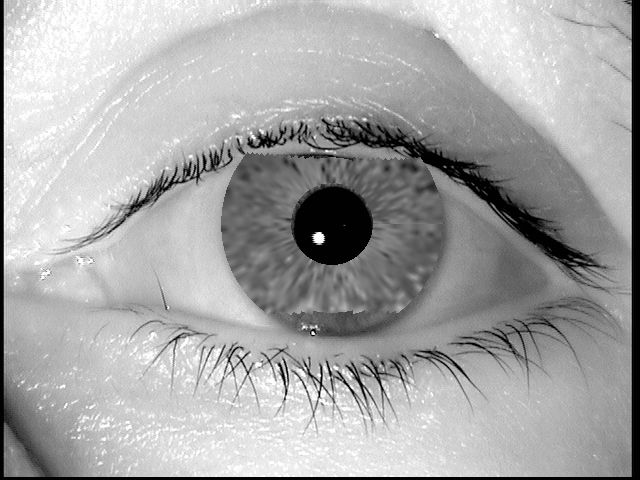
\includegraphics[scale=0.2]{./res/eyescan.jpg}
                \caption{before detection}
            \end{center}
        \end{figure}
      \end{column}

      \begin{column}{.5\textwidth}
        \begin{figure}
            \begin{center}
                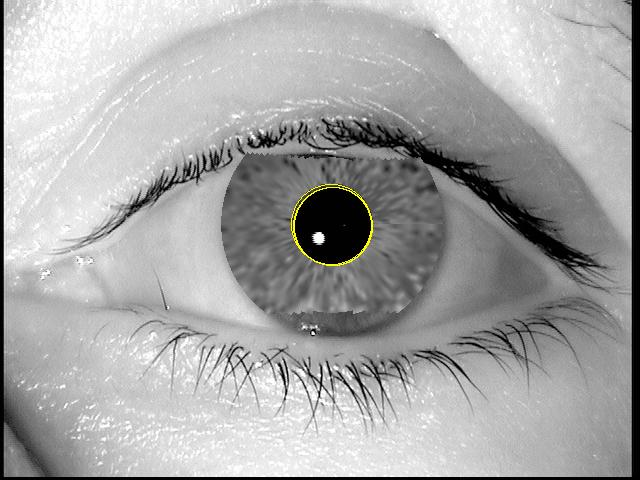
\includegraphics[scale=0.2]{./res/eyescan-detected.jpg}
                \caption{after detection}
            \end{center}
        \end{figure}
      \end{column}

    \end{columns}

    Image from: \href{http://www.wired.com/images\_blogs/threatlevel/2012/07/Iris-Image\_Galbally-Study1.jpg}{www.wired.com}
}

%%%%%%%%%%%%%%%%%%%%%%%%%%%%%%%%%%%%%%%%%%%%%%%%%%%%%%%%%%%%%%%%%%%%%%%%
%%% Algorithm
%%%%%%%%%%%%%%%%%%%%%%%%%%%%%%%%%%%%%%%%%%%%%%%%%%%%%%%%%%%%%%%%%%%%%%%%

\section{Algorithm}
\frame{
    \frametitle{Algorithm: Circular Hough Transform}

    \begin{columns}[c]

      \begin{column}{.5\textwidth}
        \begin{figure}
            \begin{center}
                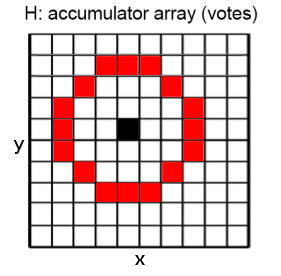
\includegraphics[scale=0.6]{./res/hough-accumulator2D-vote.png}
                \caption{2D Hough Voting Space, Single Radius}
            \end{center}
        \end{figure}
      \end{column}

      \begin{column}{.5\textwidth}

        \begin{itemize}
            \item every edge pixel (BLACK) assumes it is on the edge of a circle
            \item vote for the possible centers of the circle (RED)
            \item pixels with enough votes is detected as a circle
            \item robust, able to detect even partial circle
            \item slow, cache-unfriendly
            \item Baseline from Github repository: {\it marcbowes/Hough-Circle-Detector}
        \end{itemize}

      \end{column}

    \end{columns}

}

%%%%%%%%%%%%%%%%%%%%%%%%%%%%%%%%%%%%%%%%%%%%%%%%%%%%%%%%%%%%%%%%%%%%%%%%
%%% OPTIMIZATION
%%%%%%%%%%%%%%%%%%%%%%%%%%%%%%%%%%%%%%%%%%%%%%%%%%%%%%%%%%%%%%%%%%%%%%%%
\section{Optimization}
\frame{
    \frametitle{Optimization: Parallelization Scheme I}
    \begin{columns}[c]

      \begin{column}{.5\textwidth}
        \begin{figure}
            \begin{center}
                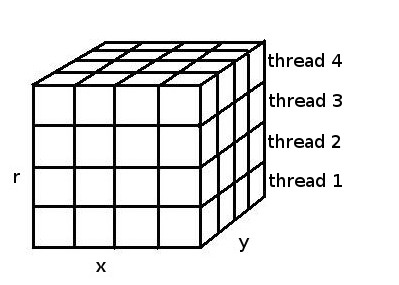
\includegraphics[scale=0.6]{./res/parallelization-scheme-1.jpg}
                \caption{parallelize by radius}
            \end{center}
        \end{figure}
      \end{column}

      \begin{column}{.5\textwidth}

        \begin{itemize}
            \item divide work by radius
            \item no shared writable data between threads
            \item no lock/synchronization required
            \item works poorly for small range of radius
        \end{itemize}

      \end{column}

    \end{columns}
}

\frame{
    \frametitle{Optimization: Parallelization Scheme II}
    \begin{columns}[c]

      \begin{column}{.5\textwidth}
        \begin{figure}
            \begin{center}
                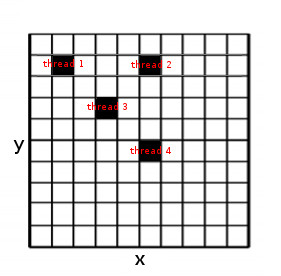
\includegraphics[scale=0.6]{./res/parallelization-scheme-2.jpg}
                \caption{parallelize by pixel}
            \end{center}
        \end{figure}
      \end{column}

      \begin{column}{.5\textwidth}

        \begin{itemize}
            \item divide work by pixels
            \item shared voting space
            \item require locks, or
            \item parallel histogram counting algorithm
        \end{itemize}

      \end{column}

    \end{columns}
}

% \frame{
%     \frametitle{Optimization: Parallelization Scheme III}
%     \begin{columns}[c]
%
%       \begin{column}{.5\textwidth}
%         \begin{figure}
%             \begin{center}
%                 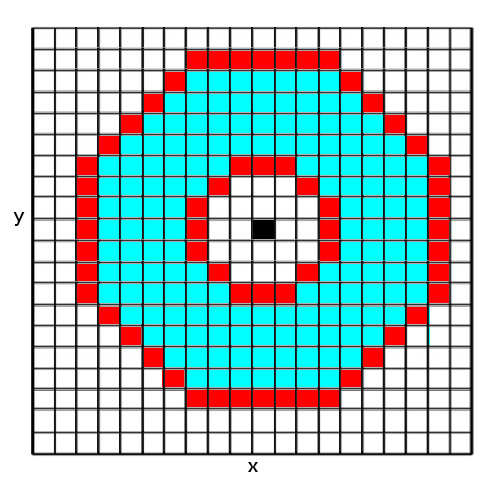
\includegraphics[scale=0.4]{./res/cache-friendly-voting.jpg}
%                 \caption{parallelize according to cache-friendly voting}
%             \end{center}
%         \end{figure}
%       \end{column}
%
%       \begin{column}{.5\textwidth}
%         Can we write our code for voting to be cache-friendly?
%
%         \begin{itemize}
%             \item Yes, but only if we squeeze the 3D hough space to 2D.
%             \item How can we change our data structure to take advantage of this?
%         \end{itemize}
%
%       \end{column}
%
%     \end{columns}
% }
%
% \frame{
%     \frametitle{Optimization: Parallelization Scheme III, Cont.}
%     \begin{columns}[c]
%
%       \begin{column}{.5\textwidth}
%         \begin{figure}
%             \begin{center}
%                 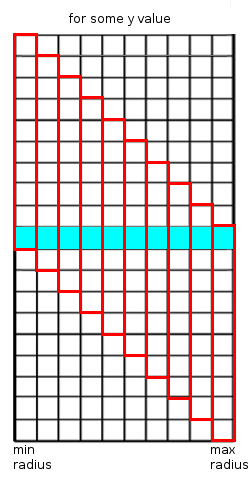
\includegraphics[scale=0.4]{./res/cache-friendly-data-structure.png}
%                 \caption{parallelize according to cache-friendly voting}
%             \end{center}
%         \end{figure}
%       \end{column}
%
%       \begin{column}{.5\textwidth}
%
%         \begin{itemize}
%             \item for each y, we create a 2D voting array
%             \item 2D voting array padded by $r_{max} - r_{min}$
%             \item x index shift by 1 for each radius
%         \end{itemize}
%
%       \end{column}
%
%     \end{columns}
% }

\frame{
    \frametitle{Optimization: Grouped Votes by Row}

    \begin{columns}[c]

      \begin{column}{.5\textwidth}
        \begin{figure}
            \begin{center}
                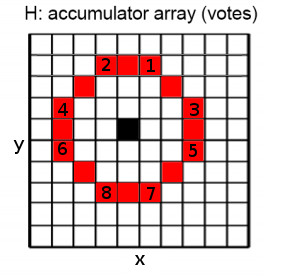
\includegraphics[scale=0.6]{./res/hough-accumulator2D-midpoint-circle-memory-access-pattern.jpg}
                \caption{Midpoint Circle Algorithm: memory access pattern}
            \end{center}
        \end{figure}
      \end{column}

      \begin{column}{.5\textwidth}
        \begin{figure}
            \begin{center}
                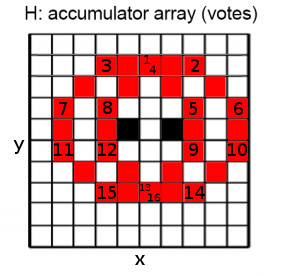
\includegraphics[scale=0.6]{./res/hough-accumulator2D-grouped-circle-memory-access-pattern.jpg}
                \caption{Grouped Voting: memory access pattern}
            \end{center}
        \end{figure}
      \end{column}

    \end{columns}
}

\frame{
    \frametitle{Optimization: Boundary Check Removal}

    \begin{columns}[c]

      \begin{column}{.5\textwidth}
        \begin{figure}
            \begin{center}
                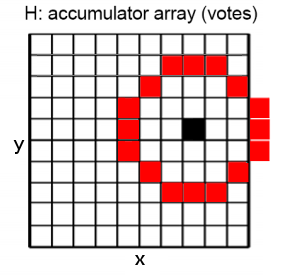
\includegraphics[scale=0.6]{./res/hough-accumulator2D-boundary-check.png}
                \caption{Out of Voting Space}
            \end{center}
        \end{figure}
      \end{column}

      \begin{column}{.5\textwidth}
        \begin{figure}
            \begin{center}
                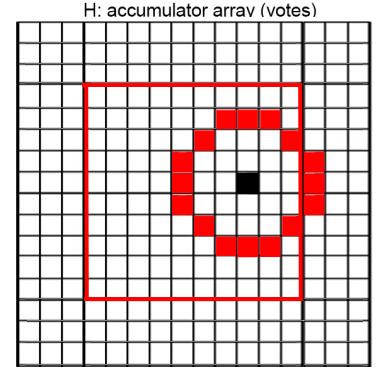
\includegraphics[scale=0.5]{./res/hough-accumulator2D-padding.png}
                \caption{Padded Voting Space}
            \end{center}
        \end{figure}
      \end{column}

    \end{columns}
}

%%%%%%%%%%%%%%%%%%%%%%%%%%%%%%%%%%%%%%%%%%%%%%%%%%%%%%%%%%%%%%%%%%%%%%%%
%%% RESULTS
%%%%%%%%%%%%%%%%%%%%%%%%%%%%%%%%%%%%%%%%%%%%%%%%%%%%%%%%%%%%%%%%%%%%%%%%
\section{Results}
\frame{
    \frametitle{Results}

    \begin{figure}
        \begin{center}
            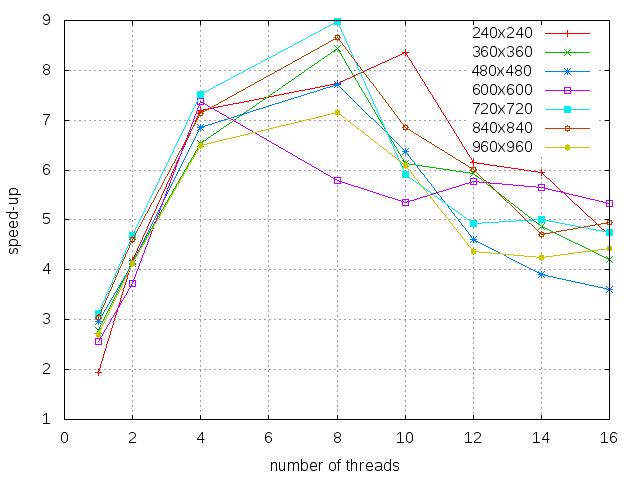
\includegraphics[scale=0.5]{./res/scalability.png}
            \caption{Scalability vs. Number of threads}
        \end{center}
    \end{figure}
}

%%%%%%%%%%%%%%%%%%%%%%%%%%%%%%%%%%%%%%%%%%%%%%%%%%%%%%%%%%%%%%%%%%%%%%%%
%%% REFERENCES
%%%%%%%%%%%%%%%%%%%%%%%%%%%%%%%%%%%%%%%%%%%%%%%%%%%%%%%%%%%%%%%%%%%%%%%%
\section{References}
\frame{
    \frametitle{References}
    \begin{thebibliography}{1}

        \bibitem{c1962method}
        H.~C, ``Method and means for recognizing complex patterns,'' Dec.~18 1962.
        \newblock US Patent 3,069,654.

        \bibitem{Kourie_anassertion-guided}
        D.~G. Kourie and B.~W. Watson, ``An assertion-guided derivation of a circle
          drawing algorithm.''

    \end{thebibliography}
}

\bibliography{bibtexdoc}
\bibliographystyle{ieeetr}

\end{document}
